\documentclass[11pt,a4paper,fleqn,notitlepage,oneside]{article}

%<--------------------------------------------------------------------------------------------------->
%<--------------------------------------------------------------------------------> 		  PACKAGES

\usepackage[utf8]{inputenc}
\usepackage{lmodern}% http://ctan.org/pkg/lm
\usepackage{indentfirst}
\usepackage{siunitx}
\usepackage{float}
\usepackage{booktabs}
\usepackage{longtable}
\usepackage[letterpaper, margin=1in]{geometry}
\usepackage{pgf}
\usepackage[margin=2.5cm]{caption}
\usepackage{graphicx}
\graphicspath{{../data/plots/summary_plots/}{../data/plots/}}

\title{Defining WFIRST Survey Parameters: \\ Computational Methods}
\author{Sol W. Courtney, Kathryn V. Johnston \& Robyn E. Sanderson \\ Columbia University Dept. Astronomy and Astrophysics}
\date{\today}

\begin{document}
\maketitle

\begin{abstract}
	This document summarizes a first look at the possible parameters of a WFIRST survey of stellar halos around the 100 most luminous galaxies within 10Mpc of us. 
	There are broadly three aims of such surveys: (i) to look at the global properties of the halos (e.g. radial profile and total content); (ii) to find structures that are signatures of recent accretion events in order to examine broad properties and variety in accretion histories (including luminosity functions, rates and orbits); (iii) to find features at widest possible separations for subsequent spectroscopic follow up in order to place potential constraints.
	For all of the above purposes, the halos should be observed to the greatest radial extent possible.
	The extent to which this is possible or interesting will depend on expected densities of the stellar halos as well as contamination by background galaxies at faint magnitudes.
	The study “observes" the Bullock/Johnston stellar halo models as a guide for expectations (could be subsequently replaced with other models - e.g. FIRE).
\end{abstract}

\begin{figure}[H]
	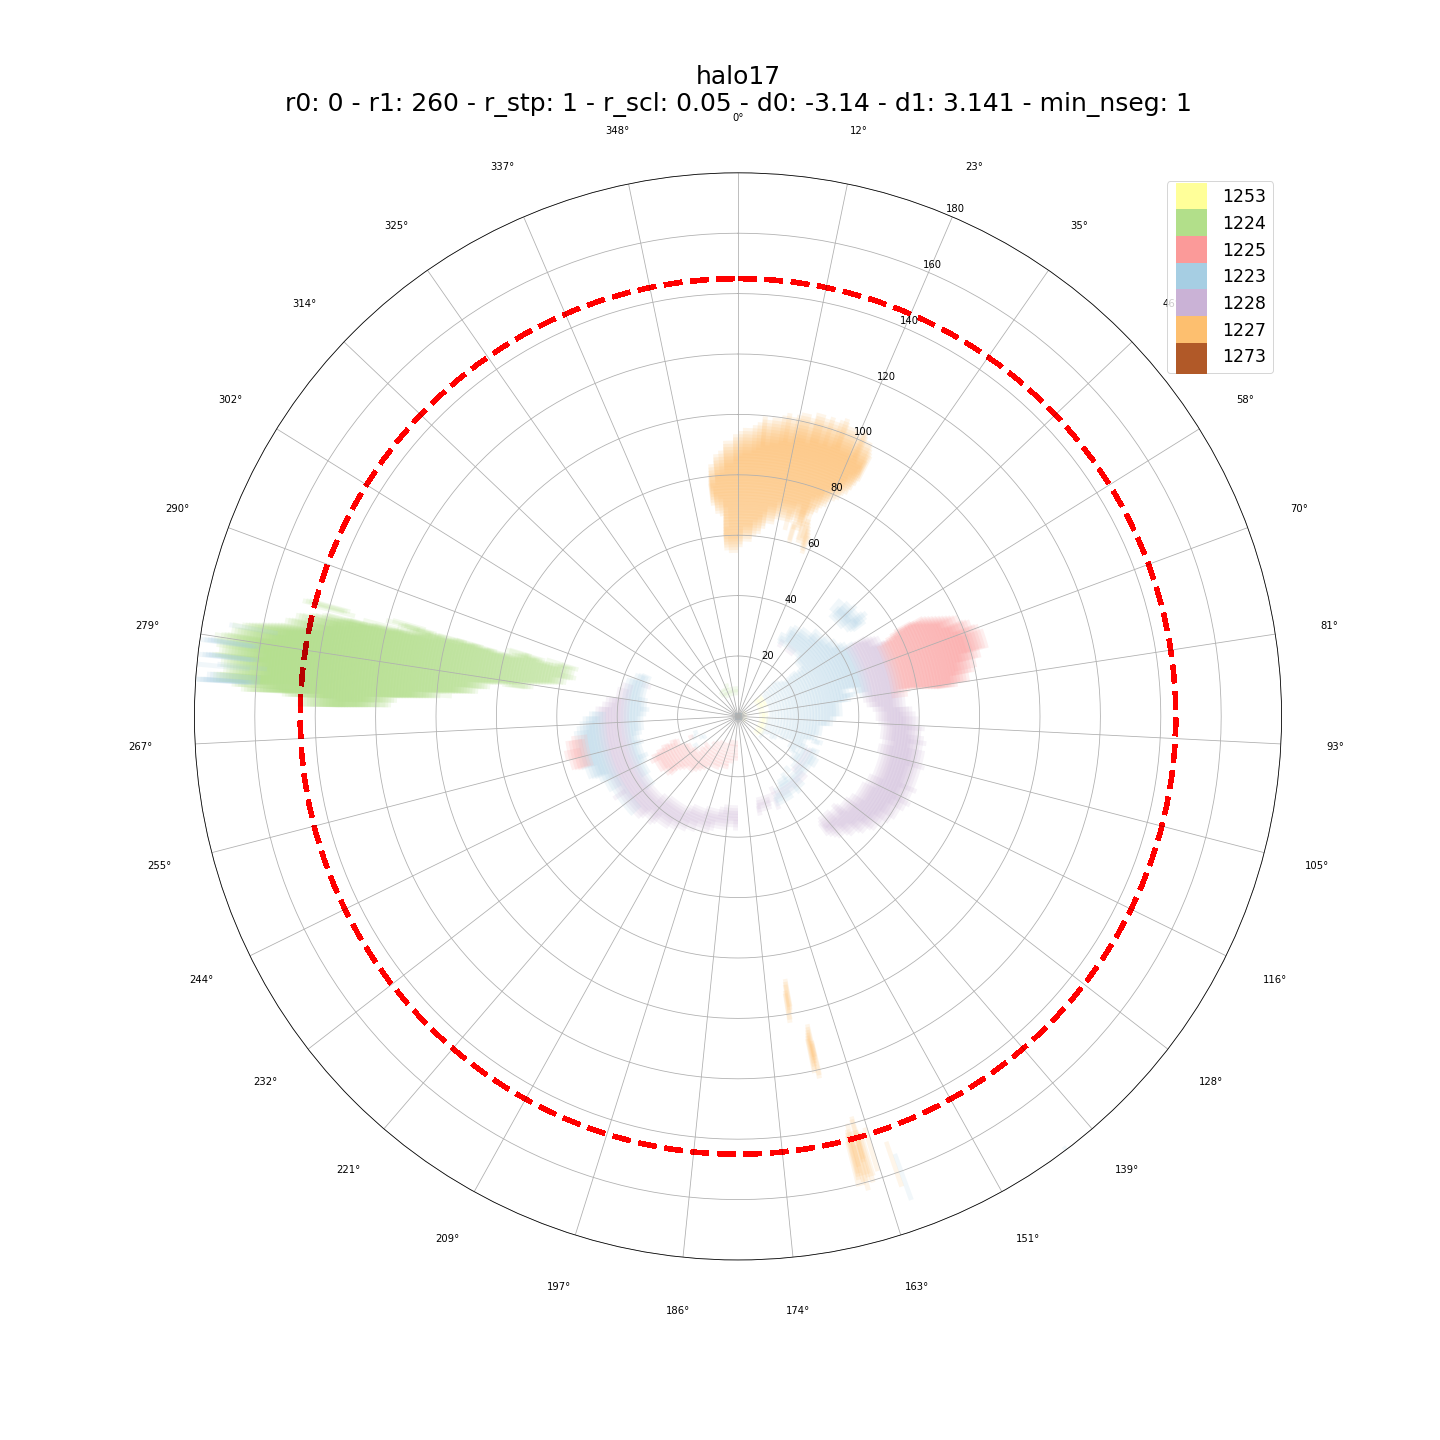
\includegraphics[width=17cm]{halo17_1.png}
	\caption{
		Halo17 skysearcher output.  Explanation
	}
	\label{fig:halo17_1}
\end{figure}

\section{Basic Idea} % (fold)
	\label{sec:basic_idea}
	Radial contrast density profile.
	Contrast against radial equivalences not the whole projection.
	The relationship between sat purity and radius.

% section basic_idea (end)

\section{Computation} % (fold)
	\label{sec:computation}
	Explain the program or process quickly

% section computation (end)

\section{General Properties} % (fold)
	\label{sec:general_properties}

	\begin{figure}[H]
		\includegraphics[width=17cm]{18_domsat_mass.png}
		\caption{
			Here we see the log10 value of the dominate satellite mass in solar mass units for each feature as a function of radius.
		}
		\label{fig:domsat_mass}
	\end{figure}

	\begin{figure}[H]
		\includegraphics[width=17cm]{19_domsat_atime.png}
		\caption{
			Here we see the accretion time of each features dominate satellite in gigayears as a function of radius.
		}
		\label{fig:domsat_atime}
	\end{figure}

% section general_properties (end)

\section{Accuracy} % (fold)
	\label{sec:accuracy}
	Each feature is referenced back to the BJ stars which compose it. 
	All the stars come with an ID tag which we can use to evaluate any features constituent stellar pops. 
	Looking at the fraction of satellite IDs present in the feature we can determine cleanliness.
	As it looks, features are more distinguishable at greater separations.

	\begin{figure}[H]
		\includegraphics[width=17cm]{16_domsat_purity.png}
		\caption{
			Here we see the fraction of satellites present in the feature as a function of radius.
			The lower the value here means an ambiguous feature.
			The higher the value means the feature will be distinguished.
		}
		\label{fig:purity}
	\end{figure}

% section accuracy (end)

\section{Numbers and Maximums} % (fold)
	\label{sec:numbers}
	Features as a function of radial displacement.
	We loose stars per unit area with radius but we gain contrast and numbers of features.

	\begin{figure}[H]
		\includegraphics[width=17cm]{23_n_features.png}
		\caption{
			Here we see the total number of registered features as a function of radius.
			Each BJ halo was used once for this plot.
			11 halos total.
		}
		\label{fig:n_features}
	\end{figure}
	%
	\begin{figure}[H]
		\includegraphics[width=17cm]{10_xbox_max.png}
		\caption{
			Here we see the maximum contrast density value as a function of radius.
			The y axis value represents how many times more stars are in the feature compared with the average number of stars per box plus or minus 1 percent radius. 
		}
		\label{fig:xbox_max}
	\end{figure}

	\begin{figure}[H]
		\includegraphics[width=17cm]{24_log10(xbox_max).png}
		\caption{
			Here we see the Log10 maximum contrast density value as above. 
		}
		\label{fig:24_log10(xbox_max)}
	\end{figure}

	\begin{figure}[H]
		\includegraphics[width=17cm]{20_Log10(n_stars).png}
		\caption{
			Here we see the log10 value of the number of stars within each feature as a function of radius. 
		}
		\label{fig:n_stars}
	\end{figure}

% section numbers (end)


\section{Summary} % (fold)
	\label{sec:summary}


	\begin{figure}[H]
		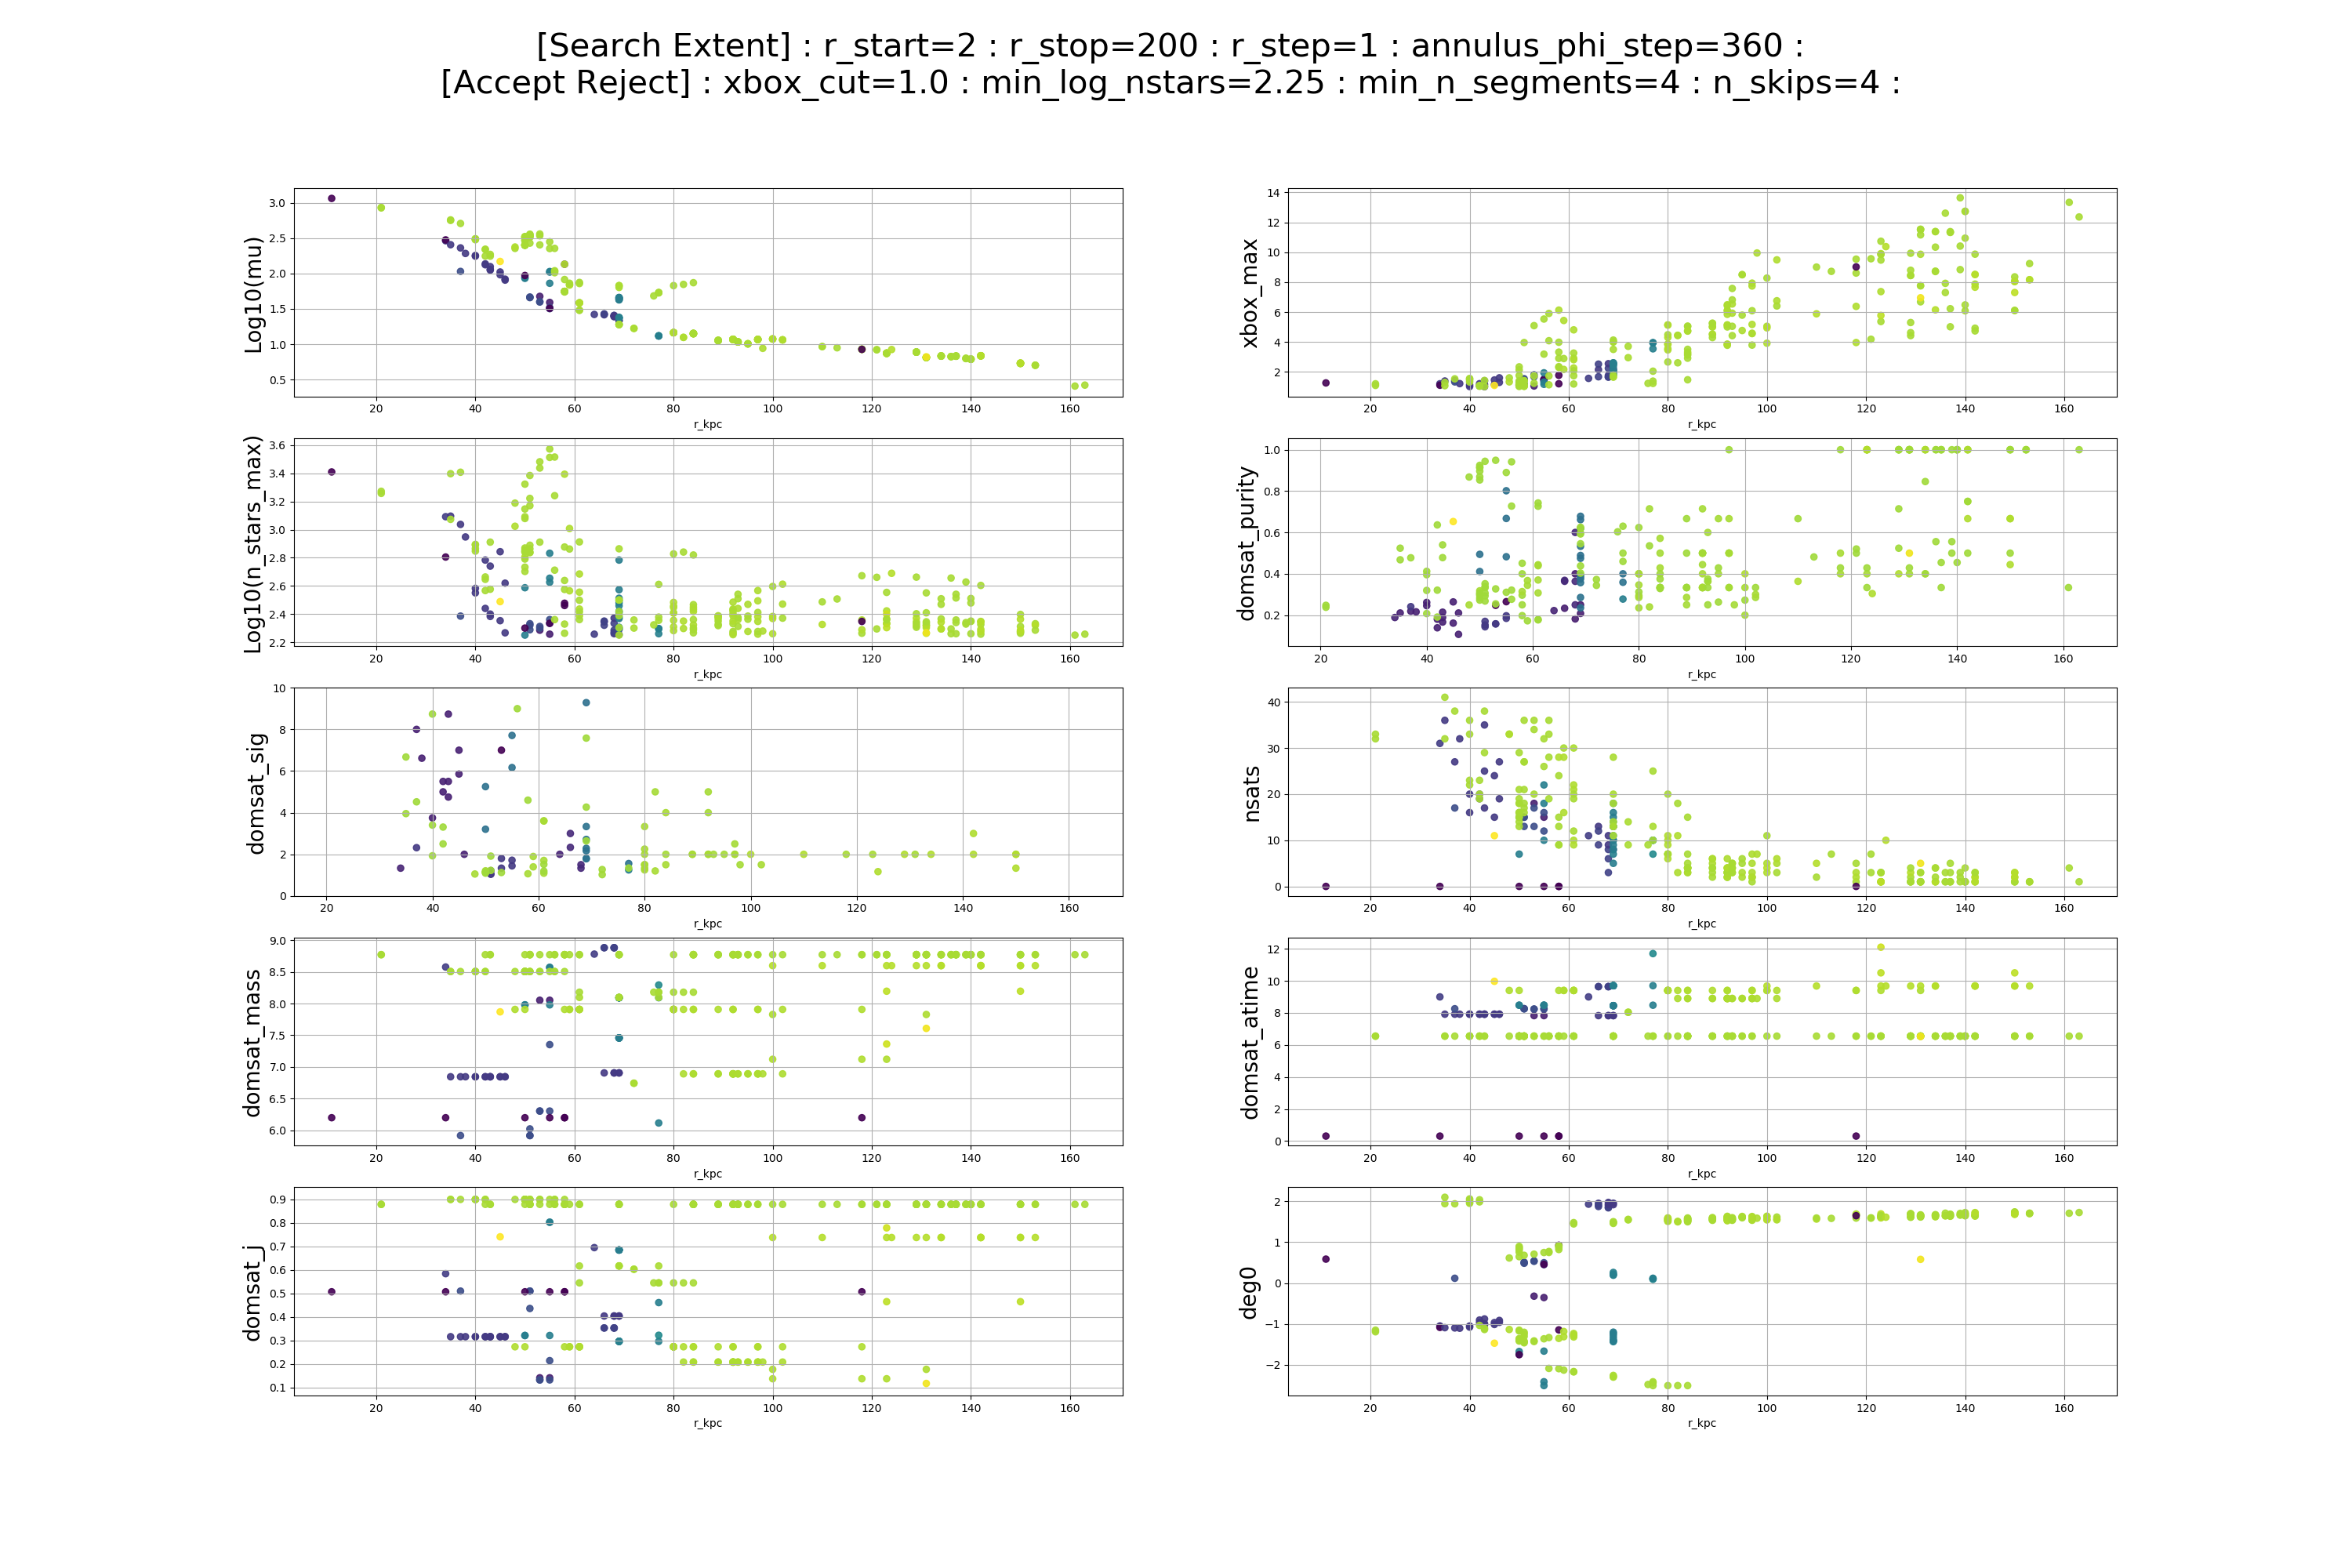
\includegraphics[width=17cm]{all_halo_summary_plot.png}
		\caption{
			Summary plot of all halos colored to halo number. 
		}
		\label{fig:all halos - summary plot}
	\end{figure}

% section summary (end)


\section{Interesting Plot Action} % (fold)
	\label{sec:interesting_plot_action}

	\begin{figure}[H]
		\includegraphics[width=17cm]{Log10(mu)_vs_Log10(n_stars)_0.png}
		\caption{
			is this good? 
		}
		\label{fig:Log10(mu)_vs_domsat_purity_5}
		\end{figure}

	\begin{figure}[H]
		\includegraphics[width=17cm]{Log10(mu)_vs_domsat_atime_1.png}
		\caption{
			? 
		}
		\label{fig:Log10(mu)_vs_domsat_purity_5}
	\end{figure}

	\begin{figure}[H]
		\includegraphics[width=17cm]{Log10(mu)_vs_domsat_purity_4.png}
		\caption{
			? 
		}
		\label{fig:Log10(mu)_vs_domsat_purity_5t}
	\end{figure}

	\begin{figure}[H]
		\includegraphics[width=17cm]{extent_vs_Log10(n_stars)_27}
		\caption{
			? 
		}
		\label{fig:extent_vs_Log10(n_stars)_27}
	\end{figure}
% section interesting_plot_action (end)

\end{document}

